\chapterimage{images/memory/leaks}

\chapter{Memory Leaks}


\section{Garbage Collection in Android}
Random-access memory (RAM) is a valuable resource in any software development environment, but it's even more valuable on a mobile operating system where physical memory is often constrained. Although both the Android Runtime (ART) and Dalvik virtual machine perform routine garbage collection, this does not mean you can ignore when and where your app allocates and releases memory. You still need to avoid introducing memory leaks, usually caused by holding onto object references in static member variables, and release any reference objects at the appropriate time as defined by lifecycle callbacks.

In this section we will focus on memory management in ART.

\section{Memory Basics}

\subsection{RAM}
RAM, which is short for random access memory, is one of the critical components of the smartphone along with the processing cores and dedicated graphics. Without RAM in any sort of computing system like this your smartphone would fail to perform basic tasks because accessing files would be ridiculously slow.

This type of memory is a middle man between the file-system, which is stored on the ROM, and the processing cores, serving any sort of information as quickly as possible. Critical files that are needed by the processor are stored in the RAM, waiting to be accessed. These files could be things such as operating system components, application data and game graphics; or generally anything that needs to be accessed at speeds faster than other storage can provide.

\subsection{ROM}
Like RAM, internal storage is critical to a smartphone’s operation; without any place to store the operating system and critical files there would be nothing for the phone to do. Even if a phone has no storage accessible to the user, there will also be some form of internal storage that stores the operating system.

Depending on the operating system loaded on the device, and the device itself, there are multiple storage chips inside the device. These chips may then be partitioned into several areas for different purposes, such as application storage, cache and system files. Normally the chip that stores the system files is called the ROM for read-only memory; however this is a bit of a misnomer as the memory here can actually be modified through system updates, just not by the end user.

\subsection{Stack Memory}
Stack memory in Android is used to store datatypes, function calls and reference variables for objects (the handle to objects).
Its contains short-lived (weak) references for objects stored in the heap memory. Whenever a function is called, a block of memory is reserved for that function and its local primitive values and reference to other objects stored inside that functions. When the function execution ends, the function block space will be free and available for other methods.

\subsection{Heap Memory}
Heap memory  in Android is used for storing Objects and java classes. When we  create an object it will take space in heap memory. Android’s memory heap is a generational one, meaning that there are different buckets of allocations that it tracks, based on the expected life and size of an object being allocated. For example, recently allocated objects belong in the young generation. When an object stays active long enough, it can be promoted to an older generation, followed by a permanent generation.

Each heap generation has its own dedicated upper limit on the amount of memory that objects there can occupy. Any time a generation starts to fill up, the system executes a garbage collection event in an attempt to free up memory. The duration of the garbage collection depends on which generation of objects it's collecting and how many active objects are in each generation.

\subsection{Shared versus private memory}
There are common framework classes, assets and native libraries that are utilized by all apps. TO save memory, Android uses shared memory for those assets.

Private memory is memory thas is used just by your app and not used by other apps. 

\subsubsection{Zygote}
Zygote \footnote{The zygote's genome is a combination of the DNA in each gamete, and contains all of the genetic information necessary to form a new individual. In multicellular organisms, the zygote is the earliest developmental stage.} is the method Android uses to start apps. Rather than having to start each new process from scratch and loading the whole system and the Android framework afresh each time you want to start an app, it does that process only once, and then stops at that point. In this initialization nothing app-specific happens. Then, when you want to start an app, the Zygote process forks, and the child process continues where it left off, loading the app itself into the VM.

\subsection{Dirty Memory vs. Clean Memory}
DIrty memory nis memory that is only stored in the RAM. Clean memory consists of items in RAM that are also saved on the disk. 

One of the main feature of the ART runtime is that apps are compiled on install. On devices running ART the app code is compiled at install and ready on disk. Because now the app code in memory is now by definition clean, memory management in ART is improved.

\section{Garbage collection}
garbage collection (GC) is a form of automatic memory management. The garbage collector, or just collector, attempts to reclaim garbage, or memory occupied by objects that are no longer in use by the program. 

The basic principles of garbage collection are to find data objects in a program that cannot be accessed in the future, and to reclaim the resources used by those objects.

The overall strategy consists of determining which objects should be garbage collected by tracing which objects are reachable by a chain of references from certain root objects, and considering the rest as garbage and collecting them.

ART has a few different GC plans that consist of running different garbage collectors. The default plan is the CMS (concurrent mark sweep). Mainly ART uses a  non-moving generational garbage collector. It scans only the portion of the heap that was modified since the last GC and can reclaim only the objects allocated since the last GC. In addition to the CMS plan, ART performs heap compaction when an app changes process state to a jank-imperceptible process state (e.g. background or cached). The goal of this compaction is to reduce memory usage of backgrounded apps. Currently, the event that triggers heap compaction is ActivityManager process-state changes. When an app goes to background, it notifies ART the process state is no longer jank “perceptible.” This enables ART do things that cause long application thread pauses, such as compaction and monitor deflation. 

\section{How much memory is used by an App}
\subsection{adb shell dumpsys meminfo}
The biggest consumers of memroy are bitmaps. No matter how well you have compresed the file or network transmission, PNG and JPEG files use 32 bits per pixe, meaning that an 100 x 100 pixel thumbnail can use 320.000 bits of memory.

ActivityManager.getMemoryClass will return the maximum size for you app' heap. Depending on this value, you can scale your application. 

To find out how much memory an app is using you can use \texttt{adb shell dumpsys meminfo}. 

\begin{verbatim}
eothein@eothein-Alienware-13:~/Android/Sdk/platform-tools$ adb shell dumpsys meminfo
adb server is out of date.  killing...
* daemon started successfully *
Applications Memory Usage (in Kilobytes):
Uptime: 60002338 Realtime: 170929502

Total PSS by process:
258,425K: system (pid 3763)
191,773K: com.facebook.orca (pid 21195 / activities)
162,638K: com.podcast.podcasts (pid 1513 / activities)
139,611K: com.android.systemui (pid 4144 / activities)
136,684K: com.google.android.gms (pid 29546)
112,756K: com.facebook.katana (pid 17090 / activities)
106,035K: com.sec.android.inputmethod (pid 7578)
104,495K: com.samsung.android.bixby.agent (pid 8652)
100,113K: com.lastpass.lpandroid (pid 22401 / activities)
97,899K: com.twitter.android (pid 2244)
87,537K: com.sec.android.app.launcher (pid 5387 / activities)
78,493K: com.google.android.gms.persistent (pid 5172)
77,809K: be.hogent.jensbuysse.metartaff (pid 1059 / activities)

\end{verbatim}

Proportional Set Size (PSS) is the total memory used by the app, which is the private memory together with the shared memory.

You can also add the PID number to the meminfo command.
\begin{verbatim}
eothein@eothein-Alienware-13:~/Android/Sdk/platform-tools$ adb shell dumpsys meminfo 1059
Applications Memory Usage (in Kilobytes):
Uptime: 60276648 Realtime: 171203812

** MEMINFO in pid 1059 [be.hogent.jensbuysse.metartaff] **
Pss  Private  Private  SwapPss     Heap     Heap     Heap
Total    Dirty    Clean    Dirty     Size    Alloc     Free
------   ------   ------   ------   ------   ------   ------
Native Heap     4552     4540        0     5626    22528    16537     5990
Dalvik Heap     4230     4208        0    10399    31791    19075    12716
Dalvik Other     1025     1024        0      712                           
Stack      272      272        0      136                           
Ashmem        4        4        0        0                           
Other dev        4        0        4        0                           
.so mmap     2539      120      360     2516                           
.apk mmap      347        0       64        0                           
.ttf mmap      110        0       36        0                           
.dex mmap     1392     1328       64     3016                           
.oat mmap     2365        0      328        0                           
.art mmap     1067      752        0      378                           
Other mmap       19        4        4        0                           
EGL mtrack    28368    28368        0        0                           
Unknown      124      124        0      408                           
TOTAL    46418    40744      860    23191    54319    35612    18706

App Summary
Pss(KB)
------
Java Heap:     4960
Native Heap:     4540
Code:     2300
Stack:      272
Graphics:    28368
Private Other:     1164
System:    28005

TOTAL:    46418       TOTAL SWAP PSS:    23191

Objects
Views:       42         ViewRootImpl:        1
AppContexts:        3           Activities:        1
Assets:       14        AssetManagers:        2
Local Binders:       12        Proxy Binders:       24
Parcel memory:        4         Parcel count:       16
Death Recipients:        0      OpenSSL Sockets:        0

SQL
MEMORY_USED:        0
PAGECACHE_OVERFLOW:        0          MALLOC_SIZE:        0

\end{verbatim} 

This is the memory usage of the app while it is in the foreground. This way we can break down how the memory allocation is distributed over the components of our application. 

The second table is showing information about things that are using mempory: view count, asset count and the number of activities. If for some reason these numbers are high, or by rerunning the command get bigger you likely have a memory issue to investigate. 

\subsection{adb shell dumpsys procstats}
Android 4.4 KitKat introduced a new system service called procstats that helps you better understand how your app is using the RAM resources on a device. Procstats makes it possible to see how your app is behaving over time — including how long it runs in the background and how much memory it uses during that time. It helps you quickly find inefficiencies and misbehaviors in your app that can affect how it performs, especially when running on low-RAM devices. In the following example we see the memory usage for the last three hours.

\begin{verbatim}
adb shell dumpsys procstats --hours 3 be.hogent.jensbuysse.metartaff
AGGREGATED OVER LAST 3 HOURS:
System memory usage:
SOff/Norm: 4 samples:
Cached: 99MB min, 146MB avg, 184MB max
Free: 20MB min, 29MB avg, 41MB max
ZRam: 0,00 min, 0,00 avg, 0,00 max
Kernel: 721MB min, 731MB avg, 741MB max
Native: 194MB min, 208MB avg, 231MB max
SOn /Norm: 32 samples:
Cached: 94MB min, 156MB avg, 304MB max
Free: 12MB min, 31MB avg, 62MB max
ZRam: 0,00 min, 0,00 avg, 0,00 max
Kernel: 706MB min, 754MB avg, 779MB max
Native: 34MB min, 70MB avg, 219MB max

Per-Package Stats:
* be.hogent.jensbuysse.metartaff / u0a307 / v1:
* be.hogent.jensbuysse.metartaff / u0a307 / v1:
TOTAL: 5,3% (68MB-55MB-80MB/41MB-60MB-75MB over 4)
Top: 5,3% (68MB-55MB-80MB/41MB-60MB-75MB over 4)
Bg TOTAL: 4,3% (38MB-38MB-38MB/9,0MB-9,0MB-9,0MB over 1)
(Last Act): 1,7% (38MB-38MB-38MB/9,0MB-9,0MB-9,0MB over 1)
(Cached): 2,6%

Summary:
* be.hogent.jensbuysse.metartaff / u0a307 / v1:
TOTAL: 5,3% (68MB-55MB-80MB/41MB-60MB-75MB over 4)
Top: 5,3% (68MB-55MB-80MB/41MB-60MB-75MB over 4)
Bg TOTAL: 4,3% (38MB-38MB-38MB/9,0MB-9,0MB-9,0MB over 1)
(Last Act): 1,7% (38MB-38MB-38MB/9,0MB-9,0MB-9,0MB over 1)
(Cached): 2,6%

Run time Stats:
SOff/Norm: +1h57m9s335ms
SOn /Norm: +32m35s716ms
TOTAL: +2h29m45s51ms

Memory usage:
Kernel : 736MB (252 samples)
Native : 178MB (252 samples)
Persist: 251MB (198 samples)
Top    : 116MB (816 samples)
ImpFg  : 401MB (1872 samples)
ImpBg  : 420KB (578 samples)
Service: 230MB (1610 samples)
Receivr: 299KB (1647 samples)
Home   : 24MB (88 samples)
LastAct: 13MB (776 samples)
CchAct : 29MB (72 samples)
CchCAct: 40MB (81 samples)
CchEmty: 342MB (1075 samples)
Cached : 148MB (252 samples)
Free   : 30MB (252 samples)
TOTAL  : 2,5GB
ServRst: 2,0MB (746 samples)

Start time: 2017-11-15 07:38:00
Total elapsed time: +7h6m26s29ms (partial) (swapped-out-pss) libart.so

Available pages by page size:
Zone   0       Unmovable      0    81     5     0     0     0     0     0     0     0     0
Zone   0         Movable   4826  1986   366    14     0     0     0     0     0     0     0
Zone   0     Reclaimable      1    25     1     0     0     0     0     0     0     0     0
Zone   0      HighAtomic     69    53    25    22    11     5     2     0     0     0     0
Zone   0             CMA      0     0     0     0     0     0     0     0     0     0     0
Zone   0         Isolate     21    15    17    19    15     9     5     3     0     1     0

\end{verbatim}

\section{Tools for tracking memory leaks}
\subsection{Android Profiler}
The Memory Profiler is a component in the Android Profiler that helps you identify memory leaks and memory churn that can lead to stutter, freezes, and even app crashes. It shows a realtime graph of your app's memory use, lets you capture a heap dump, force garbage collections, and track memory allocations.

To open the Memory Profiler, follow these steps:

\begin{enumerate}
	\item Click View > Tool Windows > Android Profiler (you can also click Android Profiler  in the toolbar).
	\item Select the device and app process you want to profile from the Android Profiler toolbar. If you've connected a device over USB but don't see it listed, ensure that you have enabled USB debugging.
	\item Click anywhere in the MEMORY timeline to open the Memory Profiler.
\end{enumerate}

\begin{figure}[h]
	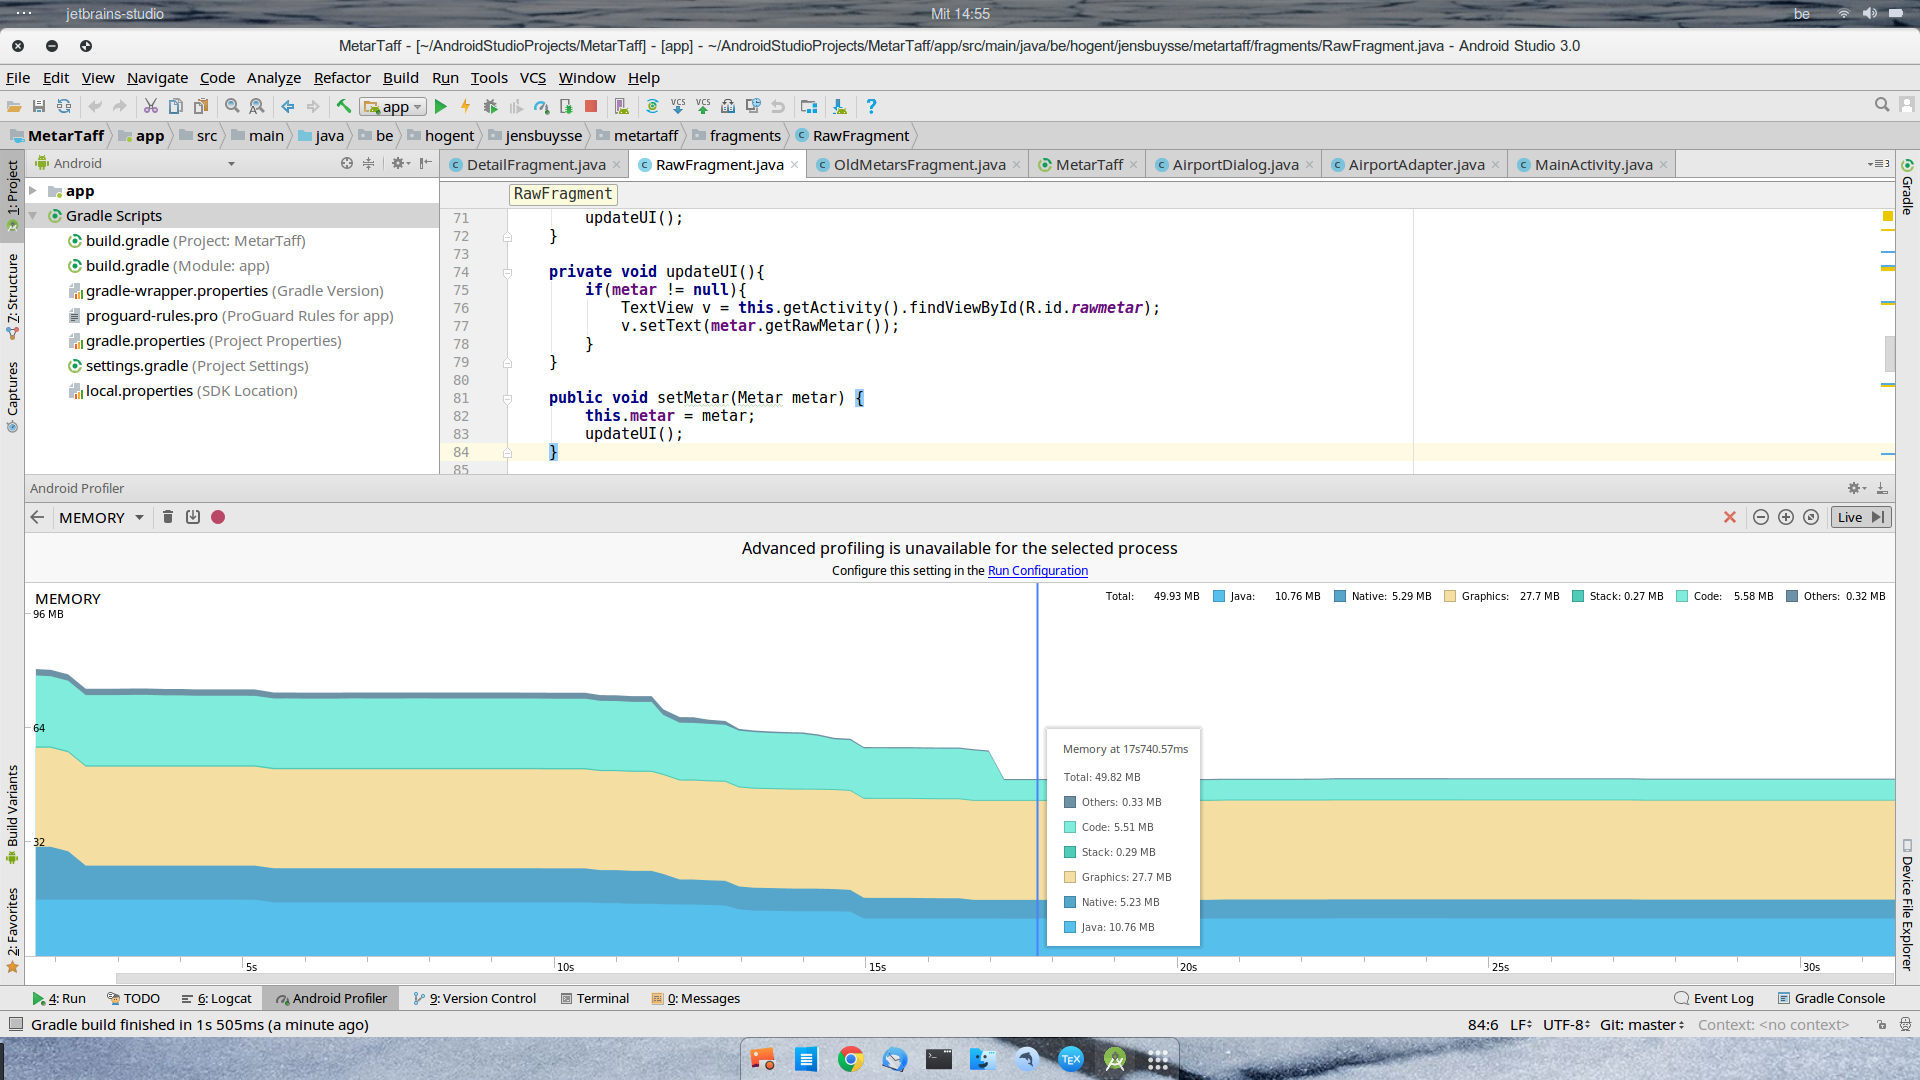
\includegraphics[width=\textwidth]{images/memory/profiler.png}
	\caption{Android provides a managed memory environment . When it determines that your app is no longer using some objects, the garbage collector releases the unused memory back to the heap}
	\label{fig:profiler}
\end{figure}

Explanation can be found \href{https://developer.android.com/studio/profile/memory-profiler.html}{here.}

\subsection{Leak Canary}
LeakCanary is an Open Source Java library to detect memory leaks in your debug builds. It is the canary in the coal mine for memory leaks: it detects memory leaks before any out-of-memory crashed are thrown. 

\section{Memory leaks: common leak patterns}
There are lots of ways you can cause a memory leak in Android. To summarize, there are mainly three categories.

\begin{enumerate}
	\item Leak activity to a static reference
	\item Leak activity to a worker thread
	\item Leak thread itself
\end{enumerate}

\subsection{Leak activity to a static reference}
A static reference lives as long as your app is in memory. An activity has lifecycles which are usually destroyed and re-created multiple times during you app’s lifecycle. If you reference an activity directly or indirectly from a static reference, the activity would not be garbage collected after it is destroyed. An activity can range from a few kilo bytes to many mega bytes depending on what contents are in it. If it has a large view hierarchy or high resolution images, it can make a large chunk of memory leaked.

\subsection{Leack activity to worker thread}
A worker thread can also out-live an Activity. If you reference an Activity directly or indirectly from a worker thread which lives longer than the Activity, you also leak the Activity object.

\subsection{Leak thread}
Every time you start a worker thread from an activity, you are responsible of managing the worker thread yourself. Because the worker thread can live longer than the Activity, you should stop the worker thread properly when the Activity is destroyed. If you forget to do so, you are risking leaking the worker thread itself.

These leaks are illustrated by \href{https://github.com/frank-tan/SinsOfMemoryLeaks}{Frank Tan}.

\newpage
\section{Exercises}
\begin{exercise}
	Add Leak Canary to the DotPict-, WhoIsIt and Metar application and find out if any of them suffer from memory leaks. Also use the profiler and the other tools which are described above. If so, you should do the following things:
	\begin{itemize}
		\item Create a new branch where you fix the problem
		\item Document the memory leak by writing a short paragraph on how the leak got constructed, how you detected it and how you solved it. Illustrate the documentation with the android profiler and abd information.
	\end{itemize}
	
\end{exercise}
